\chapter{Particles} 
The particle is taken with the fluid system, by using the velocity to add forces to the particle. The velocity and the density at the particles position is bi-linear interpolated. This velocity is multiplied with the density and with a constant. This is then applied as force to the particle. To make sure that the particle has friction, a viscous drag is also added. This is also more natural with interacting on the object.

\begin{figure}[htb!]
    \centering
    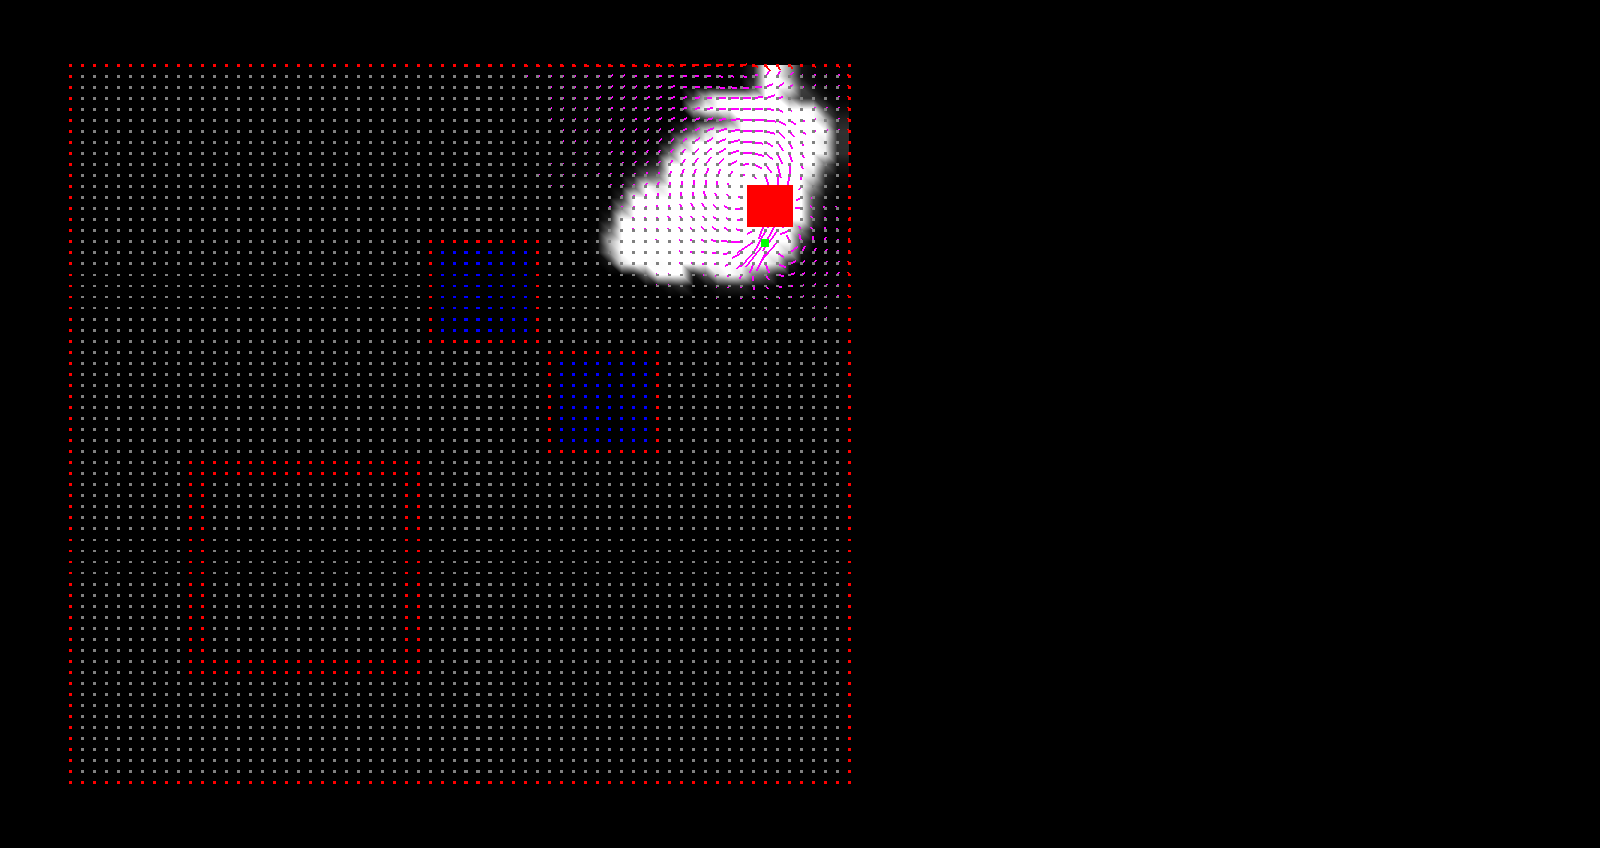
\includegraphics[width=0.6\textwidth]{images/Particle}
    \caption{A scene where a particle is taken with the fluid}
    \label{fig:Particle}
\end{figure}